%!mode::"Tex:UTF-8"
\documentclass[hyperref]{ctexart}
\usepackage{fullpage}
\usepackage{parskip}
\usepackage{physics}
\usepackage{amsmath}
\usepackage{amssymb}
\usepackage{xcolor}
%\usepackage[colorlinks,urlcolor=red,citecolor=green,anchorcolor=blue]{hyperref}
\usepackage{array}
\usepackage{longtable}
\usepackage{multirow}
\usepackage{comment}
\usepackage{graphicx}
\usepackage{cite}
%\usepackage{slashbox}
%\usepackage{intent}
\hypersetup{colorlinks,linkcolor=blue,citecolor=green}

\title{散射问题}
\author{黄应生}
\date{}

\begin{document}
\maketitle
\tableofcontents

\section{理论部分}
\subsection{Lippmann-Schwinger方程}
首先可设Hamiltonian为:
\begin{equation}\label{H}
  \hat{H}=\hat{H}_0+V(\vb{r})
\end{equation}
其中$\displaystyle\hat{H}_0=\frac{\hat{\vb{p}}^2}{2m}$,且其本征能量为$\displaystyle E_{\vb{k}}=\frac{\hbar^2\vb{k}^2}{2m}$,本征态矢为自由粒子平面波函数$\ket{\vb{k}}$。类似于在常微扰中对相互作用势做的近似,由于$V(\vb{r})$仅在很短的一段时间内有作用,可以近似看作不依赖于时间。

由含时微扰可得从$\ket{i}$跃迁到$\ket{n}$的系数也即所谓“跃迁振幅”:
\begin{equation}\label{cn}
  c_n(t)=\mel{n}{U_I(t,t_0)}{i}=\delta_{ni}-\frac{i}{\hbar}\sum_{m}\mel{n}{V}{m}\int_{t_0}^{t}e^{i\omega_{nm}t'}\mel{m}{U_I(t',t_0)}{i}\dd t
\end{equation}
其中$U_I(t,t_0)$为时间演化算符。

现取一级近似,即\eqref{cn}中的$\mel{m}{U_I(t',t_0)}{i}$为$\delta_{mi}$,且$V(\vb{r})$不显含$t$,于是得到:
\begin{equation}\label{1st order}
  \mel{n}{U_I(t,t_0)}{i}=\delta_{ni}-\frac{i}{\hbar}\mel{n}{V}{i}\int_{t_0}^{t}e^{i\omega_{nm}t'}\dd t
\end{equation}
为了处理$t$与$t_0$的渐进形式,即当$t\rightarrow\infty$且$t_0\rightarrow-\infty$的情况,定义跃迁矩阵元$T_{ni}$满足:
\begin{equation}\label{Tni}
  \mel{n}{U_I(t,t_0)}{i}=\delta_{ni}-\frac{i}{\hbar}T_{ni}\int_{t_0}^{t}e^{i\omega_{nm}t'+\varepsilon t'}\dd t
\end{equation}
其中$\varepsilon\rightarrow0^+$且$\displaystyle t\ll\frac{1}{\varepsilon}$即$\varepsilon t\ll 1$。由此当$t\rightarrow\infty$(但因为先取$\varepsilon\rightarrow0$,$\displaystyle\frac{1}{\varepsilon}$是更高阶的无穷大)时,$e^{\varepsilon t'}$趋于无穷;当$t_0\rightarrow-\infty$时,整个被积函数趋于0。

于是可以定义散射矩阵元(利用$\displaystyle\delta(x-a)=\frac{1}{2\pi}\int_{-\infty}^{\infty}e^{ip(x-a)}\dd p$):
\begin{eqnarray}\label{Sni}
  %\nonumber
  S_{ni}=\lim_{t\rightarrow\infty}\bqty{\lim_{\varepsilon\rightarrow0}\mel{n}{U_I(t,-\infty)}{i}}&=&\delta_{ni}-\frac{i}{\hbar}T_{ni}\int_{-\infty}^{\infty}e^{i\omega_{ni}t'}\dd t\\
  &=&\delta_{ni}-2\pi i \delta(E_n-E_i)T_{ni}
\end{eqnarray}

现在求解$T_{ni}$矩阵元:

首先若不做极限,式\eqref{Tni} $t_0\rightarrow-\infty$时变为(当$\ket{n}\neq\ket{i}$):
\begin{eqnarray}
  \mel{n}{U_I(t,-\infty)}{i}&=&-\frac{i}{\hbar}T_{ni}\int_{-\infty}^{t}e^{i\omega_{ni}t'+\varepsilon t'}\dd t'\\
  &=&-\frac{i}{\hbar}T_{ni}\frac{1}{i\omega_{ni}+\varepsilon}\eval{e^{(i\omega_{ni}+\varepsilon)t'}}_{-\infty}^{t}\\
  &=&-\frac{i}{\hbar}T_{ni}\frac{e^{(i\omega_{ni}+\varepsilon)t}}{i\omega_{ni}+\varepsilon}\label{nolim}
\end{eqnarray}
显然当$\ket{n}\neq\ket{i}$的限制不存在时,
\begin{equation}\label{nolim=}
  \mel{n}{U_I(t,-\infty)}{i}=\delta_{ni}+\frac{1}{\hbar}T_{ni}\frac{e^{(i\omega_{ni}+\varepsilon)t}}{-\omega_{ni}+i\varepsilon}
\end{equation}
若不做一级近似,即回到式\eqref{cn}中,则有:
\begin{equation}\label{cn1}
  \mel{n}{U_I(t,-\infty)}{i}=\delta_{ni}-\frac{i}{\hbar}\sum_{m}V_{nm}\int_{-\infty}^{t}e^{i\omega_{nm}t'}\mel{m}{U_I(t',-\infty)}{i}\dd t
\end{equation}
其中$V_{nm}=\mel{n}{V}{m}$。将\eqref{nolim=}代入\eqref{cn1}的被积函数中,得到一个多项式,第一项明显为$\delta_{ni}$,第二项为:
\begin{eqnarray}\label{6.1.25}
  -\frac{i}{\hbar}\sum_{m}V_{nm}\int_{-\infty}^{t}e^{i\omega_{nm}t'}\delta_{mi}\dd t‘&=&-\frac{i}{\hbar}V_{ni}\int_{-\infty}^{t}e^{i\omega_{ni}t'}\dd t‘\\
  &=&-\frac{1}{\hbar}V_{ni}\frac{e^{i\omega_{ni}t}}{\omega_{ni}}
\end{eqnarray}
第三项为:
\begin{eqnarray}
% \nonumber % Remove numbering (before each equation)
  -\frac{i}{\hbar}\sum_{m}V_{nm}\int_{-\infty}^{t}e^{i\omega_{nm}t'}\frac{1}{\hbar}T_{ni}\frac{e^{(i\omega_{ni}+\varepsilon)t}}{-\omega_{ni}+i\varepsilon}\dd t’&=& -\frac{i}{\hbar^2}\sum_{m}V_{nm}\frac{T_{mi}}{-\omega_{mi}+i\varepsilon}\int_{-\infty}^{t}e^{i\omega_{nm}t'+i\omega_{mi}t'+\varepsilon t'}\dd t'\\
   &=&  -\frac{i}{\hbar^2}\sum_{m}V_{nm}\frac{T_{mi}}{-\omega_{mi}+i\varepsilon}\int_{-\infty}^{t}e^{i\omega_{ni}t'+\varepsilon t'}\dd t'\\
   &=& -\frac{i}{\hbar^2}\frac{e^{(i\omega_{ni}+\varepsilon)t}}{i\omega_{ni}+\varepsilon}\sum_{m}V_{nm}\frac{T_{mi}}{-\omega_{mi}+i\varepsilon}
\end{eqnarray}
将多项式与\eqref{nolim=}对比,得到($\varepsilon$是小量):
\begin{eqnarray}
% \nonumber % Remove numbering (before each equation)
  T_{ni} &=& V_{ni}+\frac{1}{\hbar}\sum_{m}V_{nm}\frac{T_{mi}}{-\omega_{mi}+i\varepsilon} \\
   &=& V_{ni}+\sum_{m}V_{nm}\frac{T_{mi}}{E_i-E_m+i\hbar\varepsilon}
\end{eqnarray}
将$T_{ni}$展成以下形式:
\begin{equation}\label{Tni1}
  T_{ni}=\sum_j\mel{n}{V}{j}\braket{j}{\psi^{(+)}}=\mel{n}{V}{\psi^{(+)}}
\end{equation}
于是有:
\begin{equation}\label{}
  \mel{n}{V}{\psi^{(+)}}=\mel{n}{V}{i}+\sum_{m}\mel{n}{V}{m}\frac{\mel{m}{V}{\psi^{(+)}}}{E_i-E_m+i\hbar\varepsilon}
\end{equation}
上式左乘$\ket{n}$并对所有$n$求和,得到:
\begin{eqnarray}\label{}
  \ket{\psi^{(+)}}&=&\ket{i}+\sum_{m}\ket{m}\frac{\mel{m}{V}{\psi^{(+)}}}{E_i-E_m+i\hbar\varepsilon}\\
  &=&\ket{i}+\sum_{m}\frac{1}{E_i-E_m+i\hbar\varepsilon}\ket{m}\mel{m}{V}{\psi^{(+)}}
\end{eqnarray}
即:
\begin{equation}\label{Lip}
  \ket{\psi^{(+)}}=\ket{i}+\frac{1}{E_i-E_m+i\hbar\varepsilon}{V}\ket{\psi^{(+)}}
\end{equation}
上式即为Lippmann-Schwinger方程(这里只考虑正向的$t$)。
\subsection{散射截面}
根据含时微扰,跃迁速率为:
\begin{equation}\label{w}
  w(i\rightarrow n)=\dv{t}\abs{\mel{n}{U_I(t,-\infty)}{i}}^2
\end{equation}
明显$\ket{n}\neq\ket{i}$时上式才有意义,由\eqref{nolim}可以得到:
\begin{equation}\label{w1}
  w(i\rightarrow n)=\dv{t}\bqty{\frac{1}{\hbar^2}\abs{T_{ni}}^2\frac{e^{2\varepsilon t}}{\omega_{ni}^2+\varepsilon^2}}=\frac{1}{\hbar^2}\abs{T_{ni}}^2\frac{2\varepsilon\; e^{2\varepsilon t}}{\omega_{ni}^2+\varepsilon^2}
\end{equation}

现在对于有限的$t$,将$\varepsilon$趋于0,则可以看出,若$\omega_{ni}\neq0$,则$w\rightarrow0$。由以下关系:
\begin{eqnarray}
% \nonumber % Remove numbering (before each equation)
  \delta(x) &=& \lim_{\varepsilon\rightarrow0+}\eta_{\varepsilon}(x) \\
  \qq{(the possion kernel)}\;\;\;{\eta_{\varepsilon}}_{possion}(x) &=& \frac{1}{\pi}\frac{\varepsilon}{\varepsilon^2+x^2}=\int_{-\infty}^{\infty}e^{2\pi i\xi x-\abs{\varepsilon\xi}}\dd \xi \\
  \int_{-\infty}^{\infty}\frac{1}{\omega^2+\varepsilon^2}\dd \omega &=& \frac{\pi}{\varepsilon}
\end{eqnarray}
则可以得到:
\begin{equation}\label{del}
  \lim_{\varepsilon\rightarrow0^+}\frac{\varepsilon\; e^{2\varepsilon t}}{\omega_{ni}^2+\varepsilon^2}=\pi \delta(\omega_{ni})=\pi\hbar\delta(E_n-E_i)
\end{equation}
于是跃迁速率为:
\begin{equation}\label{}
  w(i\rightarrow n)=\frac{2\pi}{\hbar}\abs{T_{ni}}^2\delta(E_n-E_i)
\end{equation}
与时间$t$无关。上式类似于费米黄金法则,但$V_{ni}$被$T_{ni}$取代。

类似于费米黄金法则,末态能量密度$\rho(E_n)=\Delta n/\Delta E_n$,将$\dd w$对末态能量积分即可将$\delta(E_n-E_i)$转变成$\rho(E_n)$。设$\ket{i}=\ket{\vb{k}}$,$\ket{n}=\ket{\vb{k'}}$,$\abs{\ket{\vb{k}}}=\abs{\ket{\vb{k'}}}=k$,利用自由粒子平面波的箱归一化,得到下式:
\begin{eqnarray}
% \nonumber % Remove numbering (before each equation)
  E_n &=& \frac{\hbar^2\vb{k'}^2}{2m}=\frac{\hbar^2}{2m}\pqty{\frac{2\pi}{L}}^2\abs{\vb{n}}^2 \\
  \qq{于是有} \Delta E_n&=& \frac{\hbar^2}{m}\pqty{\frac{2\pi}{L}}^2\abs{\vb{n}}\Delta\abs{\vb{n}}
\end{eqnarray}
其中$\vb{n}=n_x\vu{i}+n_y\vu{j}+n_z\vu{k}$。由$\displaystyle\vb{n}=(\frac{L}{2\pi})\abs{\vb{k'}}=(\frac{L}{2\pi})k$,$L$极大,$\abs{\vb{n}}$看作$\vb{n}$空间球的半径,$\Delta\abs{\vb{n}}$为球壳厚度,可以得到球壳内能态数:
\begin{equation}\label{n}
  \Delta n=4\pi \abs{\vb{n}}^2\Delta\abs{\vb{n}}\times\frac{\dd \Omega}{4\pi}
\end{equation}
最后一项是考虑到末态所规定的立体角的部分($\ket{\vb{k'}}$本身代表粒子以动量$\vb{k'}$出射的态,是有方向的量)。

于是:
\begin{equation}\label{rho}
  \rho(E_n)=\frac{\Delta n}{\Delta E_n}=\frac{m}{\hbar^2}\pqty{\frac{L}{2\pi}}^2\abs{\vb{n}}\,\dd \Omega=\frac{mk}{\hbar^2}\pqty{\frac{L}{2\pi}}^3\dd \Omega
\end{equation}
又:
\begin{equation}\label{dw}
  \dd w=\frac{2\pi}{\hbar}\abs{T_{ni}}^2\,\delta(E_n-E_i)\rho(E_n)\dd E_n
\end{equation}
积分后得到:
\begin{equation}\label{ww}
  w=\frac{2\pi}{\hbar}\abs{T_{ni}}^2\,\rho(E_n)=\frac{mk}{\hbar^3}\frac{L^3}{(2\pi)^2}\abs{T_{ni}}^2\dd\Omega
\end{equation}

根据微分散射截面的定义:单位时间每靶粒子散射入立体角$\dd\Omega$的粒子数与入射流密度之比,可以得到微分散射截面$\displaystyle\frac{\dd\sigma}{\dd\Omega}$的值。其中入射流密度(由入射流速度$\displaystyle \vb{v}=\frac{\hbar \vb{k}}{m}$)
\begin{equation}\label{jx}
  \vb{j}(\vb{x},t)=\pqty{\frac{\hbar}{m}}\frac{\vb{k}}{L^3}
\end{equation}
于是
\begin{equation}\label{dsig}
  \frac{\dd\sigma}{\dd\Omega}=\frac{w}{j\,\dd\Omega}=\pqty{\frac{mL^3}{2\pi\hbar^2}}^2\abs{T_{ni}}^2
\end{equation}
得到微分散射截面。
\subsection{散射振幅}
由式\eqref{Lip}的Lippmann-Schwinger方程,左乘一个$\bra{\vb{x}}$之后得到积分方程:
\begin{equation}\label{Integraleq}
  \braket{\vb{x}}{\psi^{(+)}}=\braket{\vb{x}}{i}+\int\dd^3x'\mel{\vb{x}}{\frac{1}{E_i-E_m+i\hbar\varepsilon}}{\vb{x'}}\mel{\vb{x'}}{V}{\psi^{(+)}}
\end{equation}
考虑被积函数中的第一个矩阵元,定义$G(\vb{x},\vb{x'})$如下:
\begin{equation}\label{Gx}
  G(\vb{x},\vb{x'})\equiv\frac{\hbar^2}{2m}\mel{\vb{x}}{\frac{1}{E_i-E_m+i\hbar\varepsilon}}{\vb{x'}}
\end{equation}
同上插入离散的态矢$\ket{\vb{k'}}$、$\ket{\vb{k''}}$,有:
\begin{equation}\label{g1}
   G(\vb{x},\vb{x'})=\frac{\hbar^2}{2m}\sum_{\vb{k'}}\sum_{\vb{k''}}\braket{\vb{x}}{\vb{k'}}\mel{\vb{k'}}{\frac{1}{E_i-E_m+i\hbar\varepsilon}}{\vb{k''}}\braket{\vb{k''}}{\vb{x'}}
\end{equation}
将$H_0$作用于$\bra{\vb{k'}}$上,得到
\begin{equation}\label{g2}
  \mel{\vb{k'}}{\frac{1}{E_i-E_m+i\hbar\varepsilon}}{\vb{k''}}=\frac{\delta_{\vb{k'}\vb{k''}}}{E-\frac{\hbar^2\vb{k'}^2}{2m}+i\varepsilon}
\end{equation}
由坐标表象与动量表象(实际上和动量表象应相差一个$\hbar$)的变换关系
\begin{equation}\label{xk}
  \braket{\vb{x}}{\vb{k}}=\frac{e^{i\vb{k}\cdot\vb{x}}}{(2\pi)^{\frac{3}{2}}}\qquad\&\qquad\braket{\vb{k}}{\vb{x}}=\frac{e^{-i\vb{k}\cdot\vb{x}}}{(2\pi)^{\frac{3}{2}}}
\end{equation}
又令$E=\displaystyle\frac{\hbar^2k^2}{2m}$可以得到
\begin{eqnarray}\label{g3}
  G(\vb{x},\vb{x'})&=&\frac{\hbar^2}{2m}\sum_{\vb{k'}}\sum_{\vb{k''}}\frac{\delta_{\vb{k'}\vb{k''}}}{\frac{\hbar^2k^2}{2m}-\frac{\hbar^2\vb{k'}^2}{2m}+i\varepsilon}\frac{e^{i(\vb{k'}\cdot\vb{x}-\vb{k''}\cdot\vb{x'})}}{(2\pi)^3}\\
  &=&\frac{1}{(2\pi)^3}\sum_{\vb{k'}}\frac{e^{i\vb{k'}\cdot(\vb{x}-\vb{x'})}}{k^2-\vb{k'}^2+\frac{2i\varepsilon m}{\hbar^2}}
\end{eqnarray}
为方便起见,重新定义$\varepsilon$,使得
\begin{equation}\label{g4}
  G(\vb{x},\vb{x'})=\frac{1}{(2\pi)^3}\sum_{\vb{k'}}\frac{e^{i\vb{k'}\cdot(\vb{x}-\vb{x'})}}{k^2-\vb{k'}^2+i\varepsilon}
\end{equation}
$\varepsilon$仍然满足其原有性质。假设$\ket{\vb{k'}}$是连续的,也即箱归一化中的$L$趋于$\infty$(若之前的变换关系采用箱归一化),则求和变为积分:
\begin{equation}
   G(\vb{x},\vb{x'})=\frac{1}{(2\pi)^3}\int\dd^3k'\frac{e^{i\vb{k'}\cdot(\vb{x}-\vb{x'})}}{k^2-\vb{k'}^2+i\varepsilon}
\end{equation}
设$\mu\equiv\cos(\theta)$,上式变成
\begin{eqnarray}
% \nonumber % Remove numbering (before each equation)
  G(\vb{x},\vb{x'})&=& \frac{1}{(2\pi)^2}\int_0^{\infty}k'^2\dd k'\int_{+1}^{-1}\dd\mu\frac{e^{ik'\abs{\vb{x}-\vb{x'}}\mu}}{k^2-\vb{k'}^2+i\varepsilon} \\
   &=& \frac{1}{4\pi^2}\int_0^{\infty}k'^2\dd k'\frac{e^{-ik'\abs{\vb{x}-\vb{x'}}\mu}-e^{ik'\abs{\vb{x}-\vb{x'}}\mu}}{k^2-\vb{k'}^2+i\varepsilon}\frac{1}{ik'\abs{\vb{x}-\vb{x'}}}\\
   &=& \frac{1}{8\pi^2}\int_{-\infty}^{\infty}k'\dd k'\frac{e^{-ik'\abs{\vb{x}-\vb{x'}}\mu}-e^{ik'\abs{\vb{x}-\vb{x'}}\mu}}{k^2-\vb{k'}^2+i\varepsilon}\frac{1}{i\abs{\vb{x}-\vb{x'}}}
\end{eqnarray}
用留数定理求解以上积分(过程略),得到
\begin{equation}\label{g5}
   G(\vb{x},\vb{x'})=-\frac{1}{4\pi}\frac{e^{ik'\abs{\vb{x}-\vb{x'}}}}{\abs{\vb{x}-\vb{x'}}}
\end{equation}
即为亥姆霍兹方程中的格林函数:
\begin{equation}\label{helm}
  (\nabla^2+k^2)G(\vb{x},\vb{x'})=\delta^3(\vb{x}-\vb{x'})
\end{equation}

积分方程\eqref{Integraleq}于是可以写为
\begin{equation}\label{Inte2}
  \braket{\vb{x}}{\psi^{(+)}}=\braket{\vb{x}}{i}-\int\dd^3x'\frac{m}{2\hbar^2\pi}\frac{e^{ik'\abs{\vb{x}-\vb{x'}}}}{\abs{\vb{x}-\vb{x'}}}\mel{\vb{x'}}{V}{\psi^{(+)}}
\end{equation}
可以看出这与一般教科书中$\displaystyle e^{ikz}+f(\theta)\frac{e^{ikr}}{r}$的形式已经很接近了。

若假设$V(\vb{r})$是短程(局域)势,则在坐标表象中它是对角的。即有
\begin{equation}\label{Vxx}
  \mel{\vb{x'}}{V}{\vb{x''}}=V(\vb{x'})\delta^3(\vb{x'}-\vb{x''})
\end{equation}
于是
\begin{eqnarray}\label{xV}
  \mel{\vb{x'}}{V}{\psi^{(+)}}&=&\int\dd x''^3\mel{\vb{x'}}{V}{\vb{x''}}\braket{\vb{x''}}{\psi^{(+)}}\\
  &=&\int\dd x''^3V(\vb{x'})\delta^3(\vb{x'}-\vb{x''})\braket{\vb{x''}}{\psi^{(+)}}\\
  &=&V(\vb{x'})\braket{\vb{x'}}{\psi^{(+)}}
\end{eqnarray}
代入\eqref{Inte2},得到
\begin{equation}\label{Inte3}
  \braket{\vb{x}}{\psi^{(+)}}=\braket{\vb{x}}{i}-\frac{m}{2\pi\hbar^2}\int\dd^3x'\frac{e^{ik'\abs{\vb{x}-\vb{x'}}}}{\abs{\vb{x}-\vb{x'}}}V(\vb{x'})\braket{\vb{x'}}{\psi^{(+)}}
\end{equation}

观察上式,其中的$\vb{k}$可以看做粒子入射的波矢,$\vb{k'}$可以看做粒子出射的波矢,$\vb{x}$是空间原点到探测器的位矢,$\vb{x‘}$是空间原点到空间内另一点的位矢,$\abs{\vb{x}-\vb{x'}}$是空间内另一点到探测器的相对位矢。探测器处的波函数可以看做是空间内所有点的作用总和也即是对$\vb{x'}$的积分。

现先作几个近似。方便起见,令$\abs{\vb{x}}=r$,$\abs{\vb{x'}}=r'$,且$r\gg r'$两位矢夹角为$\alpha$。有
\begin{eqnarray}
% \nonumber % Remove numbering (before each equation)
  \abs{\vb{x}-\vb{x'}} &=& \sqrt{r^2+r'^2-2rr'\cos(\alpha)} \\
   &=& r\pqty{1+\frac{r'^2}{r^2}-2\frac{r'}{r}\cos(\alpha)}^{\frac{1}{2}} \\
   &\approx& r\pqty{1-2\frac{r'}{r}\cos(\alpha)}^{\frac{1}{2}}\\
   \text{一阶泰勒展开:}&\approx& r-\vu{r}\cdot\vb{x'}
\end{eqnarray}
$\vu{r}$被定义为$\vb{x}$方向的单位矢量:$\displaystyle\vu{r}\equiv\frac{\vb{x}}{r}$,同样有$\vb{k}=k\vu{r}$。而
\begin{equation}\label{er}
  \frac{e^{ik'\abs{\vb{x}-\vb{x'}}}}{\abs{\vb{x}-\vb{x'}}}\approx\frac{e^{ikr}}{r}e^{-i\vb{k'}\cdot\vb{x'}}
\end{equation}

当初态设为平面波波矢$\ket{i}=\ket{\vb{k}}$时,式\eqref{Inte3}于是变成
\begin{eqnarray}
% \nonumber % Remove numbering (before each equation)
 \label{Inte4} \braket{\vb{x}}{\psi^{(+)}} &=& \braket{\vb{x}}{i}-\frac{m}{2\pi\hbar^2}\int\dd^3x'\frac{e^{ikr}}{r}e^{-i\vb{k'}\cdot\vb{x'}}V(\vb{x'})\braket{\vb{x'}}{\psi^{(+)}} \\
 \label{Inte5}  &=& \frac{1}{(2\pi)^{\frac{3}{2}}}\bqty{e^{-i\vb{k}\cdot\vb{x}}+f(\vb{k},\vb{k'})\frac{e^{ikr}}{r}}
\end{eqnarray}
而当$z$轴方向取$\vb{k}$方向,即从$z$轴入射时,上式变为
\begin{equation}\label{fth}
  \braket{\vb{x}}{\psi^{(+)}}=\frac{1}{(2\pi)^{\frac{3}{2}}}\bqty{e^{-ikz}+f(\vb{k},\vb{k'})\frac{e^{ikr}}{r}}
\end{equation}

由\eqref{Inte4}和\eqref{Inte5},散射振幅$f(\vb{k},\vb{k'})$的具体形式如下:
\begin{eqnarray}
% \nonumber % Remove numbering (before each equation)
  f(\vb{k},\vb{k'}) &=& -\frac{m(2\pi)^{\frac{3}{2}}}{2\pi\hbar^2}\int\dd^3x'e^{-i\vb{k'}\cdot\vb{x'}}V(\vb{x'})\braket{\vb{x'}}{\psi^{(+)}} \\
   &=& -\frac{m(2\pi)^3}{2\pi\hbar^2}\int\dd^3x'\braket{\vb{k'}}{\vb{x'}}V(\vb{x'})\braket{\vb{x'}}{\psi^{(+)}} \\
   \label{fkfinal}&=& -\frac{m(2\pi)^2}{\hbar^2}\mel{\vb{k'}}{V}{\psi^{(+)}}
\end{eqnarray}
将之与\eqref{dsig}相对比,得到
\begin{equation}\label{dsigf}
  \frac{\dd \sigma}{\dd\Omega}=\abs{f(\vb{k},\vb{k'})}^2
\end{equation}
\subsection{Born近似}
大部分的推导已经在上一节完成。由\eqref{Tni1}可得
\begin{equation}\label{T}
  \mel{\vb{k'}}{V}{\psi^{(+)}}=\mel{\vb{k'}}{T}{\vb{k}}
\end{equation}
又可写为
\begin{equation}\label{TV}
  T\ket{i}=V\ket{\psi^{(+)}}
\end{equation}
将\eqref{Lip}式Lippmann-Schwinger方程代入\eqref{TV}中,可得
\begin{equation}\label{TV1}
  T\ket{i}=V\ket{i}+V\frac{1}{E_i-E_m+i\hbar\varepsilon}{V}\ket{\psi^{(+)}}
\end{equation}
即为(迭代后)
\begin{eqnarray}
% \nonumber % Remove numbering (before each equation)
  T &=& V+V\frac{1}{E_i-E_m+i\hbar\varepsilon}{V}\ket{\psi^{(+)}}\bra{i} \\
   &=& V+V\frac{1}{E_i-E_m+i\hbar\varepsilon}{V}+V\frac{1}{E_i-E_m+i\hbar\varepsilon}V\frac{1}{E_i-E_m+i\hbar\varepsilon}{V}\ket{\psi^{(+)}}\bra{i} \\
   &=& V+V\frac{1}{E_i-E_m+i\hbar\varepsilon}{V}+V\frac{1}{E_i-E_m+i\hbar\varepsilon}V\frac{1}{E_i-E_m+i\hbar\varepsilon}{V}+\dots
\end{eqnarray}

取一级近似,则$T=V$。于是$\mel{\vb{k'}}{V}{\psi^{(+)}}=\mel{\vb{k'}}{V}{\vb{k}}$,即$\ket{\psi^{(+)}}=\ket{\vb{k}}$。

散射振幅$f(\vb{k},\vb{k'})$为
\begin{eqnarray}
% \nonumber % Remove numbering (before each equation)
  f(\vb{k},\vb{k'}) &=& -\frac{m(2\pi)^{\frac{3}{2}}}{2\pi\hbar^2}\int\dd^3x'e^{-i\vb{k'}\cdot\vb{x'}}V(\vb{x'})\braket{\vb{x'}}{\psi^{(+)}} \\
   &=& -\frac{m(2\pi)^{\frac{3}{2}}}{2\pi\hbar^2}\int\dd^3x'e^{-i\vb{k'}\cdot\vb{x'}}V(\vb{x'})\braket{\vb{x'}}{\vb{k}} \\
   &=& -\frac{m}{2\pi\hbar^2}\int\dd^3x'e^{-i(\vb{k'}-\vb{k})\cdot\vb{x'}}V(\vb{x'})
\end{eqnarray}
此即Born近似的形式。

设$\vb{q}=\vb{k}-\vb{k'}$,则上式变为
\begin{equation}\label{f2}
  f(\vb{k},\vb{k'})=-\frac{m}{2\pi\hbar^2}\int\dd^3x'e^{i\vb{q}\cdot\vb{x'}}V(\vb{x'})
\end{equation}
若是中心力场,则有($\displaystyle q=2k\sin(\frac{\theta}{2})$)
\begin{equation}\label{f3}
  f(\theta)=-\frac{2m}{\hbar^2}\frac{1}{2iq}\int_0^{\infty}\frac{e^{iqr}-e^{-iqr}}{r}V(r)r^2\dd r
\end{equation}
即为
\begin{equation}\label{f4}
  f(\theta)=-\frac{2m}{\hbar^2q}\int_0^{\infty}V(r)r\sin(qr)\dd r
\end{equation}
\subsection{分波法和相移}
分波法的基本思想是根据角动量守恒将入射波与反射波按不同的角动量分离开,对每个分波单独处理。首先先对平面波进行分析:

对于自由粒子平面波(即本征态为$\ket{\vb{k}}$),可以将其展开为$H_0$、$L^2$、$L_z$的共同本征态$\ket{E,l,m}$的组合($\ket{E,l,m}$即为自由粒子球面波,对所有的$l$是一组正交归一的完备基)。对$\ket{E,l,m}$,明显有:
\begin{equation}\label{elm}
  \braket{E',l',m'}{E,l,m}=\delta_{ll'}\delta_{mm'}\delta(E-E')
\end{equation}
可设$\ket{\vb{k}}$到$\ket{E,l,m}$表象的变换关系可分离变量为:
\begin{equation}\label{kelm}
  \braket{\vb{k}}{E,l,m}=g_{lE}(k)Y_l^m(\vu{k})
\end{equation}
以下证明这一形式可行:对$z$方向的$\ket{\vb{k}}$,由
\begin{equation}\label{lz}
  L_z\ket{\vb{k}}=(xp_y-yp_x)\ket{k\vu{z}}=0
\end{equation}
可以得到
\begin{equation}\label{m}
  \braket{E',l',m'}{k\vu{z}}=0 \qq{当}m'\neq0
\end{equation}
所以$\ket{k\vu{z}}$可以展开为:
\begin{equation}\label{kz}
  \ket{k\vu{z}}=\sum_{l'}\int\dd E'\ket{E',l',m'=0}\braket{E',l',m'=0}{k\vu{z}}
\end{equation}
引入旋转算符$D(\alpha=\phi,\beta=\theta,\gamma=0)$(以欧拉角定义),则
\begin{equation}\label{kkz}
  \ket{\vb{k}}=D(\alpha=\phi,\beta=\theta,\gamma=0)\ket{k\vu{z}}
\end{equation}
于是有
\begin{eqnarray}
% \nonumber % Remove numbering (before each equation)
  \braket{E,l,m}{\vb{k}} &=& \sum_{l'}\int\dd E'\mel{E,l,m}{D(\alpha=\phi,\beta=\theta,\gamma=0)}{E',l',m'=0}\braket{E',l',m'=0}{k\vu{z}} \\
   &=& \sum_{l'}\int\dd E'\delta_{ll'}\delta_{mm'}\delta(E-E')D_{m0}^{(l')}\braket{E',l',m'=0}{k\vu{z}} \\
   &=& D_{m0}^{(l)}\braket{E,l,m=0}{k\vu{z}}
\end{eqnarray}
$\braket{E,l,m=0}{k\vu{z}}$不依赖于$\vb{k}$的方向,也即$\theta$和$\phi$。根据
\begin{equation}\label{Ylm}
  {Y_l^{m}}^*(\theta,\phi)=\sqrt{\frac{2l+1}{4\pi}}D_{m0}^{(l)}(\alpha=\phi,\beta=\theta,\gamma=0)
\end{equation}
可以认为
\begin{equation}\label{gle4}
  \braket{E,l,m=0}{k\vu{z}}=\sqrt{\frac{2l+1}{4\pi}}g_{lE}^*(k)
\end{equation}
所以证明了式\eqref{kelm}的形式。

若要确定$g_{lE}(k)$的形式,首先$\ket{E,l,m}$满足:
\begin{equation}\label{schr}
  (H_0-E)\ket{E,l,m}=0
\end{equation}
将$(H_0-E)$作用于$\bra{\vb{k}}$上
\begin{equation}\label{h0ek}
  \bra{\vb{k}}(H_0-E)=(\frac{\hbar^2k^2}{2m}-E)\bra{\vb{k}}
\end{equation}
右乘$\ket{E,l,m}$
\begin{equation}\label{elmkh0e}
  \bra{\vb{k}}(H_0-E)\ket{E,l,m}=(\frac{\hbar^2k^2}{2m}-E)\bra{\vb{k}}\ket{E,l,m}=0
\end{equation}
根据$\braket{\vb{k}}{E,l,m}$的已知形式,且当$\frac{\hbar^2k^2}{2m}=E$时其不能为0。可以看出$g_{lE}(k)$中应当有一项$\displaystyle\delta(\frac{\hbar^2k^2}{2m}-E)$存在,所以
\begin{equation}\label{gle2}
  g_{lE}(k)=N\delta(\frac{\hbar^2k^2}{2m}-E)
\end{equation}
为确定系数$N$,回到\eqref{elm}:
\begin{eqnarray}
% \nonumber % Remove numbering (before each equation)
   &\phantom{=}& \braket{E',l',m'}{E,l,m}=\delta_{ll'}\delta_{mm'}\delta(E-E') \\
   &=& \int\dd^3k''\braket{E',l',m'}{\vb{k''}}\braket{\vb{k''}}{E,l,m} \\
   &=& \int k''^2\dd k'' \int\dd\Omega_{\vb{k''}}\abs{N}^2\delta(\frac{\hbar^2k''^2}{2m}-E')\delta(\frac{\hbar^2k''^2}{2m}-E)Y_l^{m}(\vb{k''}){Y_{l'}^{m}}^*(\vb{k''}) \\
   &=& \abs{N}^2\frac{mk'}{\hbar^2}\delta_{ll'}\delta_{mm'}\delta(E-E')\qq{其中}E''=\frac{\hbar^2k''^2}{2m}
\end{eqnarray}
所以
\begin{equation}\label{N}
  N=\frac{\hbar}{\sqrt{mk}}
\end{equation}
于是得到$g_{lE}(k)$的形式:
\begin{equation}\label{gle3}
  g_{lE}(k)=\frac{\hbar}{\sqrt{mk}}\delta(\frac{\hbar^2k^2}{2m}-E)
\end{equation}
因此
\begin{equation}\label{kelm2}
  \braket{\vb{k}}{E,l,m}=\frac{\hbar}{\sqrt{mk}}\delta(\frac{\hbar^2k^2}{2m}-E)Y_l^m(\vu{k})
\end{equation}
所以$\ket{\vb{k}}$在以$\ket{E,l,m}$为基矢展开的形式为
\begin{eqnarray}
% \nonumber % Remove numbering (before each equation)
  \ket{\vb{k}} &=& \sum_l\sum_m\int\dd E \ket{E,l,m}\braket{\vb{k}}{E,l,m} \\
   &=& \sum_{l=0}^{\infty}\sum_{m=-l}^{l}\eval{\ket{E,l,m}}_{E=\frac{\hbar^2k^2}{2m}}\frac{\hbar}{\sqrt{mk}}Y_l^m(\vu{k})
\end{eqnarray}
以上是动量空间的展开。

坐标空间的展开类似,坐标空间中的自由粒子球面波函数为$j_r(kr)Y_l^m(\vu{r})$(球贝塞尔函数为球面波方程的解,$n_l(kr)$由于在原点趋于无穷被舍去),变换关系:
\begin{equation}\label{xelm}
  \braket{\vb{x}}{E,l,m}=c_lj_r(kr)Y_l^m(\vu{r})
\end{equation}
又由
\begin{eqnarray}
% \nonumber % Remove numbering (before each equation)
  \braket{\vb{x}}{\vb{k}}=\frac{e^{i\vb{k}\cdot\vb{x}}}{(2\pi)^{\frac{3}{2}}} &=& \sum_l\sum_m\int\dd E \braket{\vb{x}}{E,l,m}\braket{E,l,m}{\vb{k}} \\
   &=& \sum_l\sum_m\int\dd E \;c_lj_r(kr)Y_l^m(\vu{r})\frac{\hbar}{\sqrt{mk}}\delta(\frac{\hbar^2k^2}{2m}-E){Y_l^m}^*(\vu{k}) \\
   \label{ek}&=& \sum_l\frac{2l+1}{4\pi}P_l(\vu{k}\cdot\vu{r})\frac{\hbar}{\sqrt{mk}}c_lj_r(kr)
\end{eqnarray}
上式最后一步利用了球谐函数关系:
\begin{equation}\label{YYy}
  \sum_mY_l^m(\vu{r}){Y_l^m}^*(\vu{k})=\frac{2l+1}{4\pi}P_l(\vu{k}\cdot\vu{r})
\end{equation}
同时再利用瑞利公式
\begin{equation}\label{Rayleigh}
  \frac{e^{i\vb{k}\cdot\vb{x}}}{(2\pi)^{\frac{3}{2}}}=\frac{1}{(2\pi)^{\frac{3}{2}}}\sum_l(2l+1)i^lj_r(kr)P_l(\vu{k}\cdot\vu{r})
\end{equation}
于是对比可得
\begin{equation}
c_l=\frac{i^l}{\hbar}\sqrt{\frac{2mk}{\pi}}
\end{equation}
所以坐标空间中的展开为
\begin{equation}\label{xelm2}
  \braket{\vb{x}}{E,l,m}=\frac{i^l}{\hbar}\sqrt{\frac{2mk}{\pi}}j_r(kr)Y_l^m(\vu{r})
\end{equation}

对于非自由粒子而言(即$V\neq0$),由Wigner-Eckart Theorem($T$是标量算符)
\begin{equation}\label{wet}
  \mel{E',l',m'}{T}{E,l,m}=T_l(E)\delta_{ll'}\delta_{mm'}
\end{equation}
由\eqref{fkfinal}
\begin{eqnarray}
% \nonumber % Remove numbering (before each equation)
 \nonumber f(\vb{k},\vb{k'}) &=& -\frac{m(2\pi)^2}{\hbar^2}\mel{\vb{k'}}{T}{\vb{k}} \qq{(采用一阶Born近似)}\\
  \nonumber &=& -\frac{m(2\pi)^2}{\hbar^2}\sum_l\sum_{l'}\sum_m\sum_{m'}\int\dd E\int\dd E'\braket{\vb{k'}}{E',l',m'}\mel{E',l',m'}{T}{E,l,m}\braket{E,l,m}{\vb{k}} \\
  \nonumber &=& -\frac{m(2\pi)^2}{\hbar^2}\frac{\hbar^2}{mk}\sum_l\sum_{l'}\sum_m\sum_{m'}Y_{l'}^{m'}(\vu{k'}){Y_l^m}^*(\vu{k})\eval{T_l(E)\delta_{ll'}\delta_{mm'}}_{E=\frac{\hbar^2k^2}{2m}}\\
   &=& -\frac{4\pi^2}{k}\sum_l\sum_mY_{l}^{m}(\vu{k'}){Y_l^m}^*(\vu{k})\eval{T_l(E)}_{E=\frac{\hbar^2k^2}{2m}}
\end{eqnarray}
令初态为从$z$轴方向入射的平面波,则有
\begin{equation}\label{kzzz}
  \vu{k}=\vu{z}
\end{equation}
又由\eqref{m},
\begin{eqnarray}\label{Ymk}
  Y_{l}^{m}(\vu{k})&=&Y_{l}^{0}(\vu{k'})\delta_{m0}=\sqrt{\frac{2l+1}{4\pi}}P_l(1)\delta_{m0}=\sqrt{\frac{2l+1}{4\pi}}\delta_{m0}\\
  Y_{l}^{m}(\vu{k'})&=&\sqrt{\frac{2l+1}{4\pi}}P_l(\cos\theta)\delta_{m0}
\end{eqnarray}
$f(\vb{k},\vb{k'})$与$m$彻底无关,可以完全被分解成不同$l$分波的组合了。定义分波振幅
\begin{equation}\label{flk}
  f_l(k)\equiv-\frac{\pi T_l(E)}{k}
\end{equation}
散射振幅于是被分解为
\begin{equation}\label{fkl}
  f(\vb{k},\vb{k'})=f(\theta)=\sum_{l=0}^{\infty}(2l+1)f_l(k)P_l(\cos\theta)
\end{equation}

注意到球贝塞尔函数在$r$极大时可以近似为:
\begin{equation}\label{jlr}
  j_l(kr)\xrightarrow{large\; r}\frac{e^{i(kr-l\frac{\pi}{2})}-e^{-i(kr-l\frac{\pi}{2})}}{2ikr}
\end{equation}
由\eqref{ek}且已知$\displaystyle i^l=e^{i\frac{\pi}{2}l}$,
\begin{eqnarray}
% \nonumber % Remove numbering (before each equation)
  \braket{\vb{x}}{\vb{k}} &=& \sum_l\frac{2l+1}{4\pi}P_l(\vu{k}\cdot\vu{r})\frac{\hbar}{\sqrt{mk}}\frac{i^l}{\hbar}\sqrt{\frac{2mk}{\pi}}j_r(kr) \\
   &=& \sum_lP_l(\cos\theta)\frac{2l+1}{\sqrt{8\pi^3}}i^lj_r(kr) \\
   &=& \sum_l\frac{2l+1}{(2\pi)^\frac{3}{2}}\frac{e^{ikr}-e^{-i(kr-l\pi)}}{2ikr}P_l(\cos\theta)
\end{eqnarray}
又由\eqref{fth}及上式,
\begin{eqnarray}
% \nonumber % Remove numbering (before each equation)
  \nonumber\braket{\vb{x}}{\psi^{(+)}}&\xrightarrow{large\; r}&\frac{1}{(2\pi)^{\frac{3}{2}}}\bqty{e^{-ikz}+f(\theta)\frac{e^{ikr}}{r}} \\
  \nonumber &=& \frac{1}{(2\pi)^{\frac{3}{2}}}\bqty{\sum_l(2l+1)\frac{e^{ikr}-e^{-i(kr-l\pi)}}{2ikr}P_l(\cos\theta)+\sum_{l}(2l+1)f_l(k)P_l(\cos\theta)\frac{e^{ikr}}{r}} \\
   \label{xpsi}&=& \frac{1}{(2\pi)^{\frac{3}{2}}}\sum_l(2l+1)\frac{P_l(\cos\theta)}{2ik}\bqty{(1+2ikf_l(k))\frac{e^{ikr}}{r}-\frac{e^{-i(kr-l\pi)}}{r}}
\end{eqnarray}
以上即是分波形式的波函数。

对于散射问题,对于某一球面,不考虑球内的具体波函数,进出的粒子数应守恒,更广义地说,几率守恒。因此几率流密度进出应当相等。定义
\begin{equation}\label{si}
  S_l(k)\equiv1+2ikf_l(k)
\end{equation}
则有$\abs{S_l(k)}=1$,其仅在相位上有变化。可设
\begin{equation}\label{sl}
  S_l(k)=e^{2i\delta_l}
\end{equation}
$\delta_l$隐含$k$。于是
\begin{equation}\label{fldel}
  f_l(k)=\frac{e^{2i\delta_l}-1}{2ik}=\frac{e^{i\delta_l}\sin\delta_l}{k}=\frac{1}{k\cot\delta_l-ik}
\end{equation}
对于全部的散射振幅
\begin{equation}\label{fdel}
  f(\theta)=\frac{1}{k}\sum_{l=0}^{\infty}(2l+1)e^{i\delta_l}\sin\delta_lP_l(\cos\theta)
\end{equation}

现要确定相移$\delta_l$的值。首先讨论球外情况,由于接近原点的部分已被剖去,不再存在奇点的问题,球外波函数可以写为$j_l(kr)$与$n_l(kr)$的线性组合,方便起见改写为Hankel函数的形式。对于$r$极大的情况,Hankel函数可近似为
\begin{equation}\label{Hankelr}
  h_l^{(1)}\xrightarrow{large\;r}\frac{e^{i(kr-l\frac{\pi}{2})}}{2ikr}\qquad\&\qquad h_l^{(2)}\xrightarrow{large\;r}-\frac{e^{-i(kr-l\frac{\pi}{2})}}{2ikr}
\end{equation}
将\eqref{sl}代入\eqref{xpsi}中,得到
\begin{equation}\label{xdel}
  \braket{\vb{x}}{\psi^{(+)}}=\frac{1}{(2\pi)^{\frac{3}{2}}}\sum_l(2l+1)\frac{P_l(\cos\theta)}{2ik}\bqty{e^{2i\delta_l}\frac{e^{ikr}}{r}-\frac{e^{-i(kr-l\pi)}}{r}}
\end{equation}
同时又可写为
\begin{equation}\label{xdelsy}
  \braket{\vb{x}}{\psi^{(+)}}=\frac{1}{(2\pi)^{\frac{3}{2}}}\sum_l i^l(2l+1)A_l(r)P_l(\cos\theta)
\end{equation}
其中$A_l(r)=c_l^{(1)} h_l^{(1)}+c_l^{(2)} h_l^{(2)}$。对比后得到
\begin{equation}\label{c}
  c_l^{(1)}=\frac{1}{2}e^{2i\delta_l}\qquad\&\qquad c_l^{(2)}=\frac{1}{2}
\end{equation}
于是
\begin{equation}\label{al}
  A_l(r)=e^{i\delta_l}\bqty{\cos\delta_lj_l(kr)-\sin\delta_ln_l(kr)}
\end{equation}
此后由波函数在球面上值相等以及导数(或对数导数)相等即可求出相移。注意上述$A_l(r)$仅限于刚球情况,球内势场完全不能穿透。
\section{解积分方程得到的几个短程势相移}
\subsection{球方势阱}
势场:
\begin{equation}\label{sq}
  V(r)=
\begin{cases}
  -V_0, & \;\;\;r\leq a \\
  0, &  \;\;\;r>a
\end{cases}
\end{equation}
其解析解为:
\begin{equation}\label{s}
  \delta_0=\arctan(\frac{k \tan k_1a-k_1\tan ka}{k_1+k\tan ka \tan k_1a})
\end{equation}
其中$\displaystyle k_1=\frac{\sqrt{2m(E+V_0)}}{\hbar}$,$\displaystyle k=\frac{\sqrt{2mE}}{\hbar}$。

当$l=0$,$m=1$,$\hbar=1$,$V_0=1$时,结果如下($n=1500$):
\begin{table}[!htbp]
  \centering
  \begin{tabular}{|c|c|c|c|c|c|c|}
    \hline
    % after \\: \hline or \cline{col1-col2} \cline{col3-col4} ...
    能量$E$ &0.0000001&0.00001& 0.001 & 0.1 & 10 & 1000\\\hline
    相移$\delta_0$计算值 &-0.0396357&-0.383836& 0.493181  & -1.08913 & 1.5069 & 1.09185  \\\hline
    相移$\delta_0$理论值 &-0.0350844&-0.34843& 0.42248 & -1.08401 & 1.50878 & 1.11759  \\\hline
  \end{tabular}
  \caption{不同能量对应的相移计算值与理论值}\label{sqq}
\end{table}
\subsection{$\displaystyle V(r)=\frac{\alpha}{r^2}$}
势场:
\begin{equation}\label{VVV}
  V(r)=\frac{\alpha}{r^2}
\end{equation}
根据解析解,
\begin{equation}\label{}
  \delta_l=-\frac{\pi}{2}\bqty{\sqrt{(l+\frac{1}{2})^2+\frac{2 m \alpha}{\hbar^2}}-(l+\frac{1}{2})}
\end{equation}
当$l=0$,$m=1$,$\alpha=1$,$\hbar=1$时,$\displaystyle \delta_0=-\frac{\pi}{2}\approx-1.5707963$。
\begin{table}[!htbp]
  \centering
  \begin{tabular}{|c||c|c|c|c|}
    \hline
    % after \\: \hline or \cline{col1-col2} \cline{col3-col4} ...
    \backslashbox{能量}{$r_1$} & 5 & 50 & 500 & 5000\\\hline\hline
    0.0001 & -0.0353524 & -0.350575 & -1.43881 & -1.55665  \\\hline
    0.001 & -0.11171 & -1.0149 & -1.52677 & -1.56628  \\\hline
    0.01 & -0.350575 & -1.43881 & -1.55665 & -1.56761  \\\hline
    0.1 & -1.0149 & -1.52677 & -1.56629 &   \\\hline
    1 & -1.43881 & -1.55665 & -1.5677 &   \\
    \hline
  \end{tabular}
  \caption{不同$r_1$不同能量对应的相移计算值}\label{r^2}
\end{table}\\
其结果基本与微分方程解出的一致,存在约$0.0001\%$到$2\%$的差别。
\section{对TrueV的其他几个拟合}
目前我所用的是汤川势,类似于下文尝试的高斯势,指数衰减势有同样的问题,与原始数据的吻合度较低。故在最初Fit真实势的时候我在粗略测试了指数衰减势之后就将其除以$r$,变成汤川势的形式,吻合度大大上升。
\clearpage
\begin{figure}[!htbp]
  \centering
  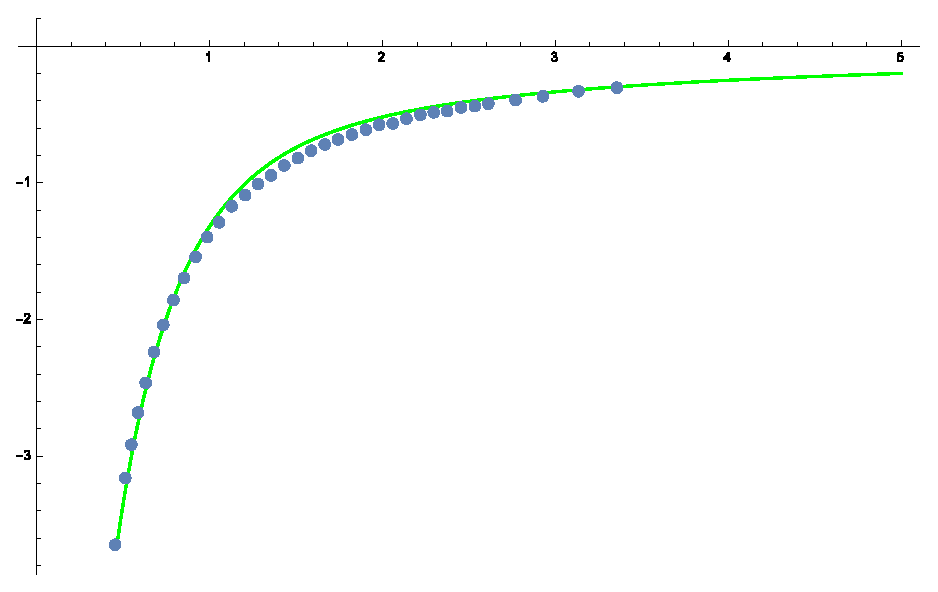
\includegraphics[width=5.2in]{Test_ReconstructLepage.eps}
  \caption{指数衰减势函数图像}
\end{figure}
\begin{figure}[!htbp]
  \centering
  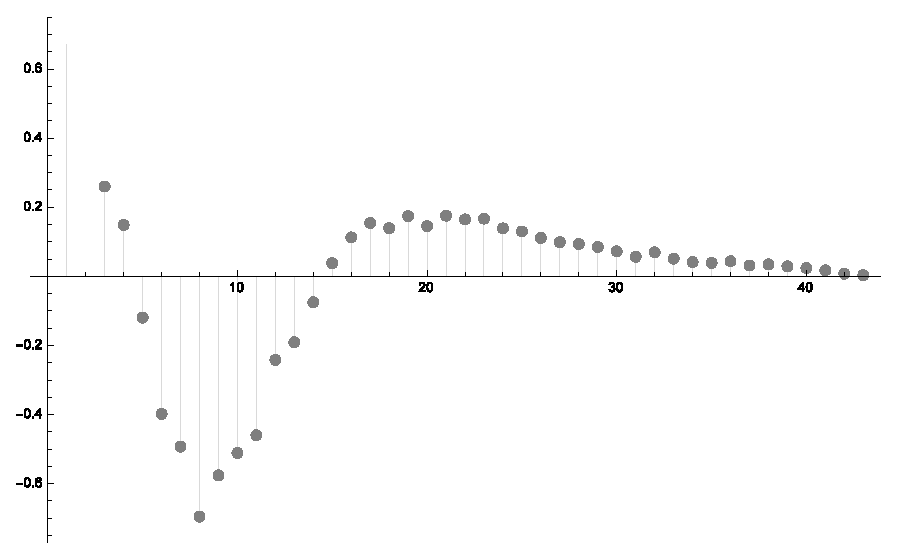
\includegraphics[width=5.2in]{Test_ReconstructLepage1.eps}
  \caption{指数衰减势在原始数据的各点上的对比(函数值平方差)}
\end{figure}
\subsection{高斯势}
势函数Fit如下:
\begin{equation}
  V_{Gauss}(r)=-2.87982 e^{-2.75997 r^2}-\frac{1}{r}
\end{equation}
于是有如下结果:
\begin{table}[!htbp]
  \centering
  \begin{tabular}{|cccccc|}
    \hline
    % after \\: \hline or \cline{col1-col2} \cline{col3-col4} ...
    能级 & 能量计算值 & Lepage能量值 & 能级 & 能量计算值 & Lepage能量值 \\
    \hline
    1S & 1.07943 & 1.28711542 & 6S & 0.0150792 & 0.0155492598 \\
    2S & 0.163432 & 0.183325753  & \dots &   & \\
    3S & 0.0658655 & 0.0703755485 & 10S & 0.0052501 & 0.00534541931 \\
    4S & 0.0354216 & 0.0371495726 & 20S & 0.00128066 & 0.00129205010 \\
    5S & 0.0220872 & 0.0229268241  &  &  &  \\
    \hline
  \end{tabular}
  \caption{高斯势S波能量对比}
\end{table}\\
其结果明显不甚乐观,误差较大,尤其在基态上较汤川势更大。

\subsection{高斯势/r}
势函数Fit如下:
\begin{equation}
  V_{Gr}(r)=-(1/r) - \frac{0.793895 e^{-0.739369 r^2}}{r}
\end{equation}
\begin{table}[!htbp]
  \centering
  \begin{tabular}{|cccccc|}
    \hline
    % after \\: \hline or \cline{col1-col2} \cline{col3-col4} ...
    能级 & 能量计算值 & Lepage能量值 & 能级 & 能量计算值 & Lepage能量值 \\
    \hline
    1S & 1.28537 & 1.28711542 & 6S & 0.0153447 & 0.0155492598 \\
    2S & 0.172902 & 0.183325753  & \dots &   & \\
    3S & 0.0682977 & 0.0703755485 & 10S & 0.00530447 & 0.00534541931 \\
    4S & 0.03638 & 0.0371495726 & 20S & 0.00128719 & 0.00129205010 \\
    5S & 0.0225585 & 0.0229268241  &  &  &  \\
    \hline
  \end{tabular}
  \caption{高斯势/r S波能量对比}
\end{table}\\
其开始的几个能级表现较好,但之后的能级误差并没有大幅度下降,在高能级不如汤川势的表现。

附其函数图像于下页。
\subsection{高斯势/r与汤川势的组合}
上述结果很自然引出了将高斯势/r与汤川势组合在一起的想法。Fit后所得结果如式\eqref{bind}。

\begin{figure}[!htbp]
  \centering
  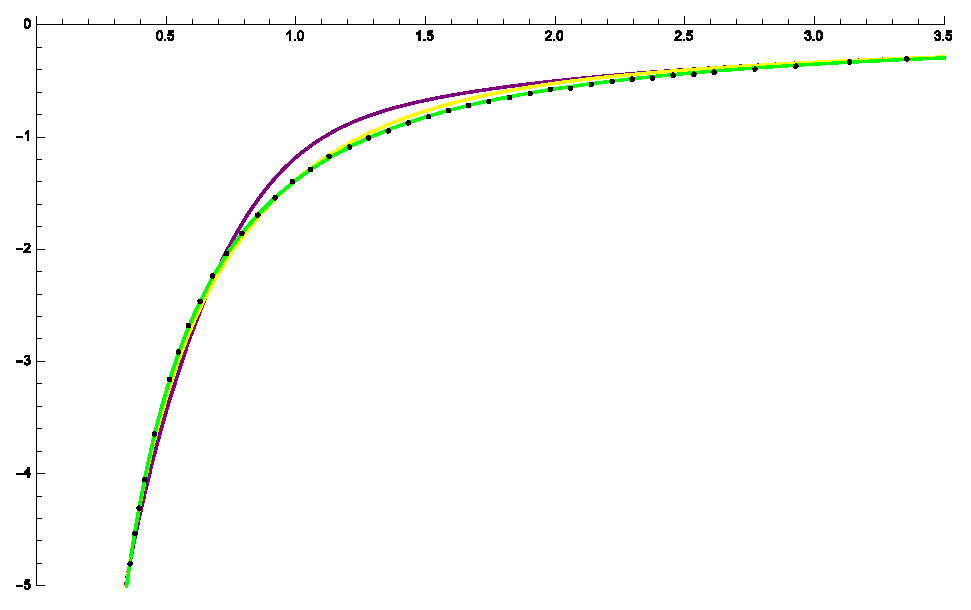
\includegraphics[width=5.2in]{Test_BindingEnergy_FitOtherwise.eps}
  \caption{汤川势与上述两势函数图像(按顺序为绿、紫、黄)}
\end{figure}

\begin{figure}[!htbp]
  \centering
  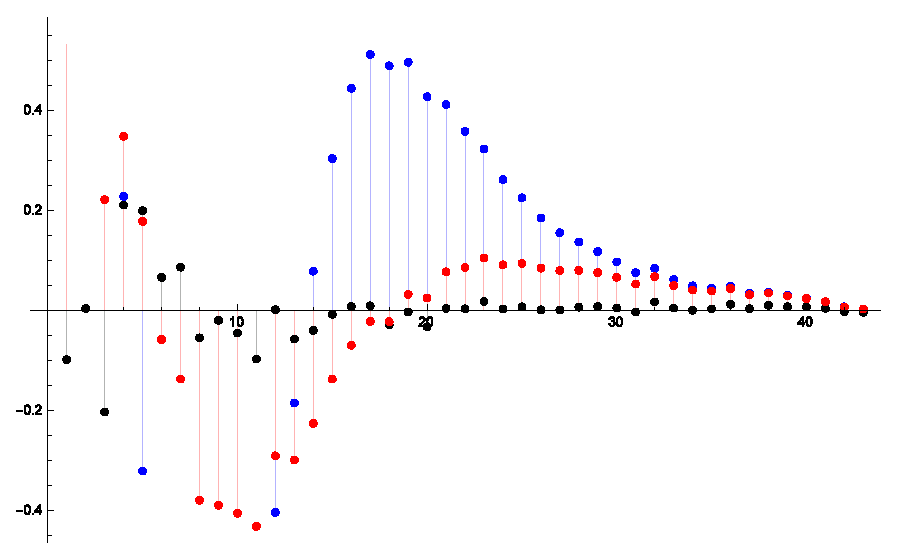
\includegraphics[width=5.2in]{Test_BindingEnergy_FitOtherwise1.eps}
  \caption{汤川势与上述两势在原始数据的各点上的对比(函数值平方差)(按顺序为黑、蓝、红)}
\end{figure}

\begin{equation}\label{bind}
  V_{bind}(x)=-\frac{0.120009 e^{-2.50727 r^2}}{r}-\frac{0.875409 e^{-0.865025 r}}{r}-\frac{1}{r}
\end{equation}
函数图像及对比见下图:
\begin{figure}[!htbp]
  \centering
  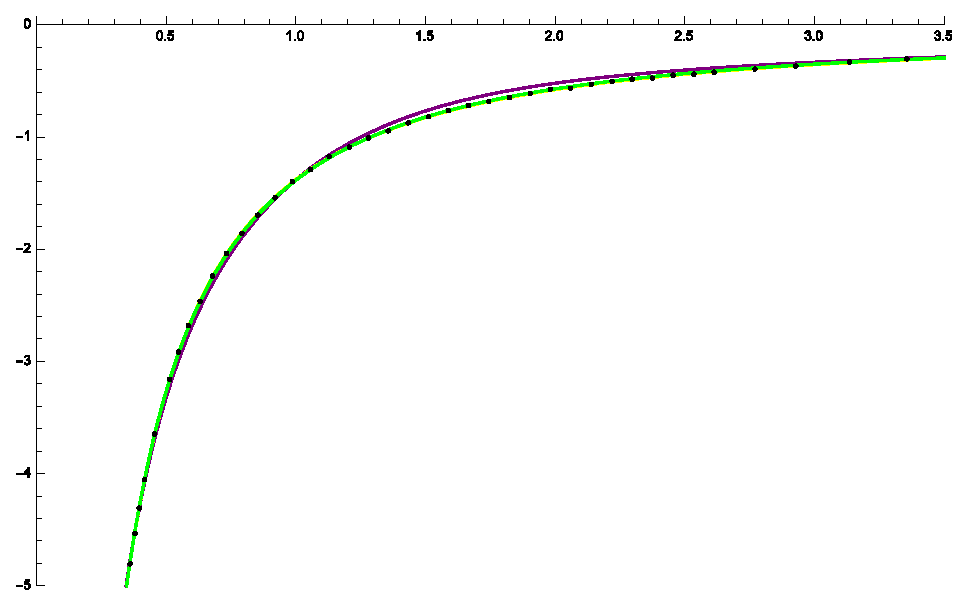
\includegraphics[width=5.2in]{Test_BindingEnergy_FitOtherwise2.eps}
  \caption{$V_{Yukawa}$、$V_{Gr}$和$V_{bind}$函数图像(按顺序为绿、紫、黄)}
\end{figure}

\begin{figure}[!htbp]
  \centering
  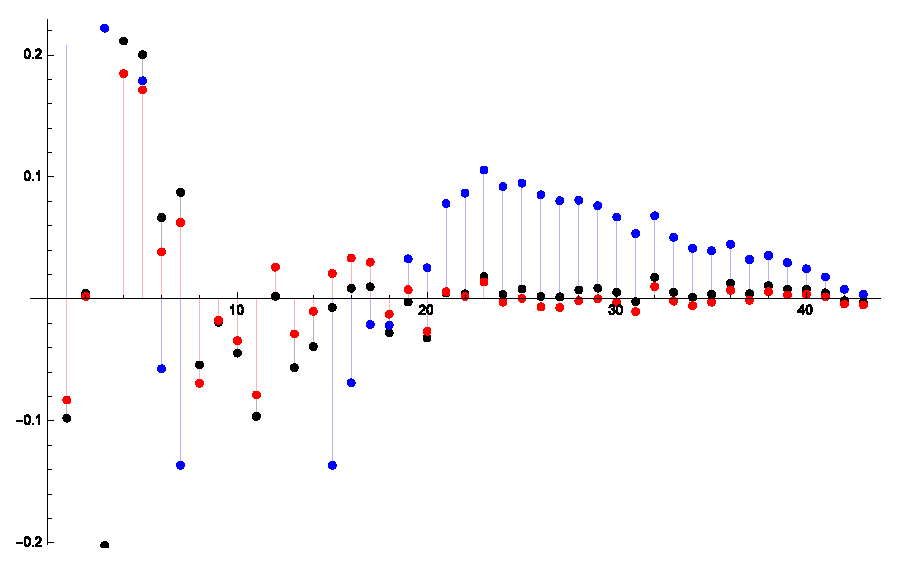
\includegraphics[width=5.2in]{Test_BindingEnergy_FitOtherwise3.eps}
  \caption{$V_{Yukawa}$、$V_{Gr}$和$V_{bind}$在原始数据的各点上的对比(函数值平方差)(按顺序为黑、蓝、红)}
\end{figure}
\clearpage
得到的能量本征值:
\begin{table}[!htbp]
  \centering
    \begin{tabular}{|cccccccc|}
    \hline
    % after \\: \hline or \cline{col1-col2} \cline{col3-col4} ...
    能级 & 能量计算值 & Lepage能量值 & 相对误差 & 能级 & 能量计算值 & Lepage能量值 & 相对误差 \\
    \hline
    1S & 1.32788 & 1.28711542 & 3.16692\% & 6S & 0.0156448 & 0.0155492598 & 0.614127\% \\
    2S & 0.188546 & 0.183325753 & 2.8473\% & \dots &   &  & \\
    3S & 0.0713584 & 0.0703755485 & 1.39658\% & 10S & 0.00536445 & 0.00534541931 & 0.35602\% \\
    4S & 0.037511 & 0.0371495726 & 0.972767\% & 20S & 0.0012943 & 0.00129205010 &0.127336\%\\
    5S & 0.0230992 & 0.0229268241 & 0.751846\% &  &  & & \\
    \hline
  \end{tabular}
  \caption{组合势S波能量对比}
\end{table}\\
除了基态较汤川势稍好外,其他均不如汤川势接近。
\section{用离散化矩阵本征值求解微分方程}
\subsection{氢原子S波束缚能}
对于氢原子S波束缚能而言,很自然地选择氢原子径向波函数作为一组正交归一的基来离散化哈密顿量:
\begin{equation}
R_n(r)=\frac{2}{a^{3/2} n^2 (2 l+1)!} \sqrt{\frac{(l+n)!}{(-l+n-1)!}} e^{-\frac{1}{2}\frac{2 r}{a n}} \left(\frac{2 r}{a n}\right)^l \,F\pqty{l-n+1,2 l+2,\frac{2 r}{n a}}
\end{equation}
由$u(r)\equiv rR(r)$,
\begin{equation}\label{ur}
  \frac{2r}{a^{3/2} n^2 (2 l+1)!} \sqrt{\frac{(l+n)!}{(-l+n-1)!}} e^{-\frac{1}{2}\frac{2 r}{a n}} \left(\frac{2 r}{a n}\right)^l \,F\pqty{l-n+1,2 l+2,\frac{2 r}{n a}}
\end{equation}
S波情况下,有
\begin{equation}\label{us}
  u(r)=\frac{2 }{a^{3/2} n^{3/2}}e^{-\frac{r}{a n}}F\pqty{1-n,2,\frac{2 r}{n}}
\end{equation}
其解明显与理论值应十分接近:
\begin{table}[!htdp]
  \centering
  \begin{tabular}{|c|c|c|c|c|c|c|}
    \hline
    % after \\: \hline or \cline{col1-col2} \cline{col3-col4} ...
    能级 & 1 & 2 & 3 & 4 & 5 & 6 \\
    \hline
    计算值 & -13.6057 & -3.40142 & -1.51174 & -0.850356 & -0.544228 & -0.377936\\
    \hline
    理论值 & -13.6057 & -3.4014 & -1.5117 & -0.8503 & -0.5442 & -0.3779 \\
    \hline
  \end{tabular}
  \caption{氢原子能级}
\end{table}
\clearpage
\subsection{势为$\displaystyle\frac{0.1}{r^2}$}
同样直接采用氢原子波函数,有:
\begin{table}[!htbp]
  \centering
  \begin{tabular}{|c|c|c|c|c|c|}
    \hline
    % after \\: \hline or \cline{col1-col2} \cline{col3-col4} ...
    能级 & 1 & 2 & 3 & 4 & 5 \\
    \hline
    NDSolve计算值 & -12.9465 & -3.34907 & -1.48763 & -0.840345 & -0.539192 \\
    \hline
    微扰值 & -12.8853 & -3.31066 & -1.48464 & -0.838833 & -0.538282 \\
    \hline
    离散矩阵本征值 & -12.8991 & -3.30893 & -1.48363 & -0.838268 & -0.53794 \\
    \hline
  \end{tabular}
  \caption{$\displaystyle V_s=\frac{0.1}{r^2}$下的能级}
\end{table}\\
结果基本比较接近,考虑到并没有解析解,二级微扰可能有影响,并不能作出更精确的判断。
\subsection{势为Lepage的真实势}
同样采用氢原子径向波函数尝试,结果如下:
\begin{table}[!htb]
  \centering
  \begin{tabular}{|cccccc|}
    \hline
    % after \\: \hline or \cline{col1-col2} \cline{col3-col4} ...
    能级 & 能量计算值 & Lepage能量值 & 能级 & 能量计算值 & Lepage能量值 \\
    \hline
    1S & 1.00113 & 1.28711542 & 6S & 0.0145071 & 0.0155492598 \\
    2S & 0.152720 & 0.183325753  & \dots &   & \\
    3S & 0.0619985 & 0.0703755485 & 10S & 0.00511407 & 0.00534541931 \\
    4S & 0.0336547 & 0.0371495726 & 20S & 0.00125987 & 0.00129205010 \\
    5S & 0.0211352 & 0.0229268241  &  &  &  \\
    \hline
  \end{tabular}
  \caption{Lepage真实势S波能量对比}
\end{table}\\
可以看出其结果并不让人满意,误差较大。\textbf{或者是否可以用该方法进行定位,而后利用原有的方法得到精确解?}当加大矩阵阶数之后,精度有小幅提升,但是主要体现在高能级上。

\subsection{NDEigensystem}
NDEigensystem是MMA 10中加入的新功能。其作用是数值求解微分方程的特征函数和特征值。该方法对于边界条件是齐次Dirichlet条件的问题十分方便,默认情况下精度略差。当然精度控制可以通过Method选项中SpatialDiscretization的离散步数进行控制。

用一维谐振子进行尝试:
\begin{equation}\label{HarmonicOscillator}
  V(x)=\frac{1}{2}x^2
\end{equation}
其解析解很明显:$\displaystyle E_n=n+\frac{1}{2}$。利用该函数解出的数值解为:
\begin{table}[!htdp]
  \centering
  \begin{tabular}{|c|c|c|c|c|c|c|}
    \hline
    % after \\: \hline or \cline{col1-col2} \cline{col3-col4} ...
    能级 & 1 & 2 & 3 & 4 & 5 & 6 \\
    \hline
    计算值 & 0.500079 & 1.50054 & 2.5019 & 3.5047 & 4.50943 & 5.51652\\
    \hline
  \end{tabular}
  \caption{一维谐振子能级}
\end{table}\\
能级越大,精度越低。

但是尝试用该方法求解氢原子能级时,我暂时没有找到将Neumann条件代入的方法。

\subsection{利用谐振子离散化方程}
该方法原本是利用谐振子写出$x$和$p$的矩阵形式(即谐振子波函数表象),然后利用这些矩阵形式将多项式形式的哈密顿量$H_0+c_1x+c_2x^2+c_3x^3\dots$转化成矩阵形式然后对角化求本征值\cite{6}。显然这种方法对于上述多项式形式的哈密顿量很方便,但是却无法应用到其他类型的势中。我尝试对其进行改造以应用于类库伦势,但是没有成功。
\subsection{差分方法}
最简单的方法如下:薛定谔方程可看做以下形式的微分方程
\begin{equation}
  \psi''(x)+f(x)\psi(x)=E\psi(x)
\end{equation}
利用欧拉方法(这是一种仅具备2阶精度的显式单步方法,实际精度不高,但是在这里可作为测试用)
\begin{equation}
\frac{d^2\psi}{d x^2}\approx \frac{\psi(x+\Delta x)+\psi(x-\Delta x)-2\psi(x)}{{\Delta x}^2}
\end{equation}
于是可以得到一个线性方程组。

对于$\psi''(x)$,它的矩阵形式于是为
$$\left[ \begin{matrix}
-2 & 1 & & 0\\
1 & \ddots & \ddots & \\
& \ddots & \ddots & 1 \\
0 & & 1 & -2 \end{matrix} \right]$$
$V(x)$就变成一个对角矩阵
$$\left[ \begin{matrix}
V(x_1) &  & & 0\\
 & \ddots & & \\
& & \ddots &  \\
0 & &  & V(x_N) \end{matrix} \right]$$
方程变成
$$\left[ \begin{matrix}
2a_0+V(x_1) & -a_0 & & 0\\
-a_0 & \ddots & \ddots & \\
& \ddots & \ddots & -a_0 \\
0 & & -a_0 & 2a_0+V(x_N) \end{matrix} \right]
\cdot
\left[\begin{matrix}
\Psi_1\\
\vdots\\
\vdots\\
\Psi_N
\end{matrix}\right]
=
E
\left[\begin{matrix}
\Psi_1\\
\vdots\\
\vdots\\
\Psi_N
\end{matrix}\right]$$
其中$\displaystyle a_0=\frac{\hbar^2}{2m(\Delta x)^2}$。如果要提高精度,就要在$\psi''(x)$的差分形式上加以改进。

目前的情况来看,用该方法解出的本征值之中甚至符号都不一致,还存在很大问题。问题可能出在边界条件的代入上。下一步应先尝试该方法解简单的本征值问题能否解出,然后进一步应用精度更高的差分方法处理。
\begin{thebibliography}{b}

\bibitem{1}
Sakurai J J, Tuan S F, Commins E D. Modern Quantum Mechanics, Second Edition. Pearson Schweiz Ag, 2013.
\bibitem{5}
曾谨言. 量子力学(卷I)(第4版)(现代物理学丛书)(精)[M]. 科学, 2007.
\bibitem{3}
Lepage P. How to Renormalize the Schrodinger Equation[J]. Nuclear Theory, 1997.
\bibitem{2}
Griffiths, David Jeffery. Introduction to quantum mechanics. Pearson Education India, 2013.
\bibitem{4}
陈鄂生. 量子力学基础教程[M]. 山东大学出版社, 2002.
\bibitem{6}
Korsch H J, Glck M. Computing quantum eigenvalues made easy[J]. European Journal of Physics, 2002, 23(23):413-426.
\end{thebibliography}

\end{document} 
